\documentclass[compress,11pt,xcolor=svgnames,aspectratio=169]{beamer}
\usetheme{Esiwace}
\usefonttheme[onlysmall]{structurebold}

%\usepackage{caption}
%\captionsetup{labelformat=empty, format=plain, labelsep=none,textfont=footnotesize}

\usepackage[utf8]{inputenc}
\usepackage[english]{babel}
\usepackage[T1]{fontenc}
\usepackage{eurosym}
\usepackage{ulem}
\usepackage{listings}
\usepackage{ragged2e}  %For \justify and \justifying, but it's not working
\usepackage{pgfgantt}
\usepackage{comment}
\usepackage{verbatim}

\newcommand{\lr}[1]{\textcolor{cyan}{LR: #1}}

\tcbuselibrary{raster}
\newcommand{\sectionIntroHidden}{
\begin{frame}{Outline}
  \tableofcontents[currentsection,subsectionstyle=hide/hide/hide]
\end{frame}
}

\DeclareGraphicsExtensions{.pdf,.png,.jpg,}
\graphicspath{{./fig/}}

\title[Input/Output and Middleware -- Lab Session]{2020 Summer School on Effective HPC for Climate and Weather \\[0.5cm] Input/Output and Middleware}
\author[Pedro, Kunkel]{Luciana Pedro, Julian Kunkel
}
\institute[WP4 Team]{Department of Computer Science, University of Reading}
\date{18 June 2020}

\begin{document}

%%%%%%%%%%%%%%%%%%%%%%%%%%%%%%%%%%%%%%%%%%%%%%%%%%%%%%%%%%%%
\begin{frame}[plain]
    \titlepage
\end{frame}

%%%%%%%%%%%%%%%%%%%%%%%%%%%%%%%%%%%%%%%%%%%%%%%%%%%%%%%%%%%%
\begin{withoutheadline}
\begin{frame}{Outline}
    \begin{centering}
    \tableofcontents[hideallsubsections]
    \end{centering}

    \disclaimer
\end{frame}
\end{withoutheadline}

% Input/Output and Middleware
% Climate and weather research is typically data-intensive and applications must utilise input/output efficiently. Often, a user struggles to assess observed performance leading to superflux attempts to tune the application and optimise performance in a wrong layer of the stack. The content of this session is twofold. Firstly, we discuss storage layers focusing on the NetCDF middleware and provide a performance model that aids users to identify inefficient I/O. Secondly, we introduce the NetCDF Climate and Forecast (CF) conventions that are often used as a standard to exchange data.

\begin{frame}[fragile]{Learning Objectives}

\begin{itemize}
\setlength\itemsep{1cm}
  \item Execute programs in C that read and write NetCDF files in a metadata-aware manner
  \item Analyze, manipulate and visualise NetCDF data
  \item Implement an application that utilizes parallel I/O to store and analyze data
\end{itemize}

\end{frame}

\section{NetCDF Files and C}

% Inserting [fragile] to be able to work with \verb

\subsection{Introduction}

\begin{frame}[fragile]{References}

\begin{itemize}
\setlength\itemsep{0.6cm}

  \item The files and data used in this presentation were collected on the Unidata website.

    \begin{itemize}
    \item \url{https://www.unidata.ucar.edu/}
    \end{itemize}

  \item All files used here are available in the following Git Repository:

    \begin{itemize}
    \item \url{https://github.com/ESiWACE/io-training}
    \end{itemize}

  \item These files are also available with the NetCDF main installation, in the directory \texttt{examples}.

  \item For more information about how to install NetCDF in your personal computer, from scratch, check Section \ref{netcdf}.

\end{itemize}

\end{frame}

\begin{frame}[fragile]{File Reference: \texttt{simple\_xy\_wr.c}}

\begin{itemize}

  \item This is an example program demonstrating a simple 2D write. It is intended to illustrate the use of the netCDF C API.\\[0.3cm]

    \begin{itemize}
      \item {\tiny \url{https://www.unidata.ucar.edu/software/netcdf/docs/simple__xy__wr_8c.html}}\\[0.3cm]
      \item {\tiny \url{https://www.unidata.ucar.edu/software/netcdf/docs/simple__xy__wr_8c_source.html}}\\[0.4cm]
    \end{itemize}

  \item Dependency graph for \verb|simple_xy_wr|:

\end{itemize}

\begin{center}
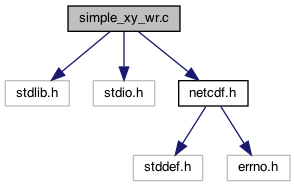
\includegraphics[scale=0.5]{fig/simple__xy__wr_8c__incl}
\end{center}

\end{frame}

\subsection{Code Analysis}

\begin{frame}[fragile]{File \texttt{simple\_xy\_wr.c}: Header and Constants Declaration}

{\tiny

\begin{verbatim}

#include <stdlib.h>
#include <stdio.h>
#include <netcdf.h>

/* This is the name of the data file we will create. */
#define FILE_NAME "simple_xy.nc"

/* We are writing 2D data, a 6 x 12 grid. */
#define NDIMS 2
#define NX 6
#define NY 12

/* Handle errors by printing an error message and exiting with a
* non-zero status. */
#define ERRCODE 2
#define ERR(e) {printf("Error: %s\n", nc_strerror(e)); exit(ERRCODE);}

int main()
{
  ...
  ...
  ...
}

\end{verbatim}

}

\end{frame}

\begin{frame}[fragile]{File \texttt{simple\_xy\_wr.c}: Variables Declaration}

{\tiny

\begin{verbatim}

...
...
...

int main()
{
  /* When we create netCDF variables and dimensions, we get back an
   * ID for each one. */
  int ncid, x_dimid, y_dimid, varid;
  int dimids[NDIMS];

  /* This is the data array we will write. It will be filled with a
   * progression of numbers for this example. */
  int data_out[NX][NY];

  /* Loop indexes, and error handling. */
  int x, y, retval;

  ...
  ...
  ...
}

\end{verbatim}

}

\end{frame}

\begin{frame}[fragile]{File \texttt{simple\_xy\_wr.c}: Creating (loading!) data}

{\tiny

\begin{verbatim}

...

int main()
{
  ...

  /* Create some pretend data. If this wasn't an example program, we
   * would have some real data to write, for example, model
   * output. */
  for (x = 0; x < NX; x++)
     for (y = 0; y < NY; y++)
    data_out[x][y] = x * NY + y;

  ...
}

\end{verbatim}

}

\end{frame}

\begin{frame}[fragile]{File \texttt{simple\_xy\_wr.c}: Creating the NetCDF file}

{\tiny

\begin{verbatim}

...

int main()
{
  ...

  /* Always check the return code of every netCDF function call. In
   * this example program, any retval which is not equal to NC_NOERR
   * (0) will cause the program to print an error message and exit
   * with a non-zero return code. */

  /* Create the file. The NC_CLOBBER parameter tells netCDF to
   * overwrite this file, if it already exists.*/
  if ((retval = nc_create(FILE_NAME, NC_CLOBBER, &ncid)))
     ERR(retval);

  ...
}

\end{verbatim}

}

\end{frame}

\begin{frame}[fragile]{File \texttt{simple\_xy\_wr.c}: Defining the dimensions}

{\tiny

\begin{verbatim}

...

int main()
{
  ...

  /* Define the dimensions. NetCDF will hand back an ID for each. */
  if ((retval = nc_def_dim(ncid, "x", NX, &x_dimid)))
     ERR(retval);
  if ((retval = nc_def_dim(ncid, "y", NY, &y_dimid)))
     ERR(retval);

  /* The dimids array is used to pass the IDs of the dimensions of
   * the variable. */
  dimids[0] = x_dimid;
  dimids[1] = y_dimid;

  ...
}

\end{verbatim}

}

\end{frame}

\begin{frame}[fragile]{File \texttt{simple\_xy\_wr.c}: Defining the variable}

{\tiny

\begin{verbatim}

...

int main()
{
  ...

  /* Define the variable. The type of the variable in this case is
   * NC_INT (4-byte integer). */
  if ((retval = nc_def_var(ncid, "data", NC_INT, NDIMS,
               dimids, &varid)))
     ERR(retval);

  /* End define mode. This tells netCDF we are done defining
   * metadata. */
  if ((retval = nc_enddef(ncid)))
     ERR(retval);

  ...
}

\end{verbatim}

}

\end{frame}

\begin{frame}[fragile]{File \texttt{simple\_xy\_wr.c}: Writing data to the file}

{\tiny

\begin{verbatim}

...

int main()
{
  ...

  /* Write the pretend data to the file. Although netCDF supports
   * reading and writing subsets of data, in this case we write all
   * the data in one operation. */
  if ((retval = nc_put_var_int(ncid, varid, &data_out[0][0])))
     ERR(retval);

  /* Close the file. This frees up any internal netCDF resources
   * associated with the file, and flushes any buffers. */
  if ((retval = nc_close(ncid)))
     ERR(retval);

  ...
}

\end{verbatim}

}

\end{frame}

\begin{frame}[fragile]{File \texttt{simple\_xy\_wr.c}: Getting SUCCESS!}

{\tiny

\begin{verbatim}

...

int main()
{
  ...

  printf("*** SUCCESS writing example file simple_xy.nc!\n");
  return 0;
}

\end{verbatim}

}

\subsection{Working and analysing the NetCDF File}

\end{frame}

\begin{frame}[fragile]{Compiling and running the file \texttt{simple\_xy\_wr.c}}

\begin{itemize}
\setlength\itemsep{0.6cm}

  \item Create (copy!) and compile the file \verb|simple_xy_wr.c|.

    \begin{itemize}
      \item {\tiny \verb|gcc -I/home/username/local/include simple_xy_wr.c -o simple_xy_wr -L/home/username/local/lib -lnetcdf|}
        \begin{itemize}
          \item \lr{What does that mean?!}
        \end{itemize}
    \end{itemize}

  \item Run the file \verb|simple_xy_wr|.

      \begin{itemize}

        \item {\tiny \verb|./simple_xy_wr|}\\

        \item {\tiny \verb|*** SUCCESS writing example file simple_xy.nc!|}\\[0.5cm]

      \end{itemize}

  \item Check that the file \verb|simple_xy.nc| is in your directory.

\end{itemize}

\end{frame}

\begin{frame}[fragile]{File Reference: \texttt{simple\_xy\_rd.c}}

\begin{itemize}

  \item This is a simple example which reads a small dummy array that was written by \verb|simple_xy_wr.c|. \\[0.3cm]

    \begin{itemize}
      \item {\tiny \url{https://www.unidata.ucar.edu/software/netcdf/docs/simple__xy__rd_8c.html}}\\[0.3cm]
      \item {\tiny \url{https://www.unidata.ucar.edu/software/netcdf/docs/simple__xy__rd_8c_source.html}}\\[0.4cm]
    \end{itemize}

  \item Dependency graph for \verb|simple_xy_rd|:

\end{itemize}

\begin{center}
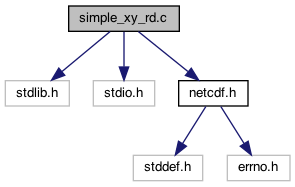
\includegraphics[scale=0.5]{fig/simple__xy__rd_8c__incl}
\end{center}

\end{frame}

\begin{frame}[fragile]{File \texttt{simple\_xy\_rd.c}}

{\tiny

\begin{verbatim}

int main()
{
   /* Open the file. NC_NOWRITE tells netCDF we want read-only access
    * to the file.*/
   if ((retval = nc_open(FILE_NAME, NC_NOWRITE, &ncid)))
      ERR(retval);

   /* Get the varid of the data variable, based on its name. */
   if ((retval = nc_inq_varid(ncid, "data", &varid)))
      ERR(retval);

   /* Read the data. */
   if ((retval = nc_get_var_int(ncid, varid, &data_in[0][0])))
      ERR(retval);

   /* Check the data. */
   for (x = 0; x < NX; x++)
      for (y = 0; y < NY; y++)
	 if (data_in[x][y] != x * NY + y)
	    return ERRCODE;

   /* Close the file, freeing all resources. */
   if ((retval = nc_close(ncid)))
      ERR(retval);
}

\end{verbatim}

}

\end{frame}

\begin{frame}[fragile]{Reading the file \texttt{simple\_xy.nc}}

\begin{itemize}
\setlength\itemsep{0.6cm}

  \item Check that the file \verb|simple_xy.nc| is in your directory.

  \item Create (copy!), compile and run the file \verb|simple_xy_rd.c|.\\[0.4cm]

        \begin{itemize}
          \item {\tiny  \verb|gcc -I/home/username/local/include simple_xy_rd.c -o simple_xy_rd -L/home/username/local/lib -lnetcdf| }\\[0.4cm]
        \end{itemize}

  \item Run the file \verb|simple_xy_rd|.

        \begin{itemize}
          \item {\tiny  \verb|./simple_xy_rd|}
          \item {\tiny  \verb|*** SUCCESS reading example file simple_xy.nc!|}
        \end{itemize}

\end{itemize}

\end{frame}

\section{NetCDF Utilities}

\begin{frame}[fragile]{\texttt{ncdump} and \texttt{ncgen}}

\begin{itemize}
\setlength\itemsep{0.6cm}

  \item \texttt{ncdump} and \texttt{ncgen} are inverses:\\[0.4cm]

  \begin{center}
  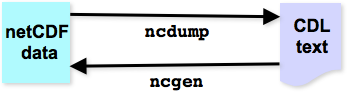
\includegraphics[scale=0.5]{fig/nc-inv}
  \end{center}

  \item Used together, \texttt{ncdump} and \texttt{ncgen} can accomplish simple netCDF manipulations with little or no programming.

\end{itemize}

\end{frame}

\begin{frame}[fragile]{Editing a NetCDF File}

\begin{itemize}
\setlength\itemsep{0.6cm}
  \item To edit metadata or data in a netCDF file:

\begin{center}
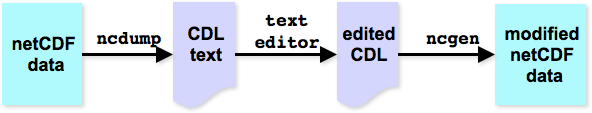
\includegraphics[scale=0.5]{fig/nc-edit}
\end{center}

  \begin{itemize}
  \setlength\itemsep{0.3cm}
    \item Use \texttt{ncdump} to convert netCDF file to CDL.
    \item Use a text editor to make desired change to CDL.
    \item Use \texttt{ncgen} to turn modified CDL back into netCDF file.
    \item \textbf{Note:} This option is not practical for huge netCDF files or if one intend to modify lots of files. For that, need to write a program using netCDF library.
  \end{itemize}

\end{itemize}

\end{frame}

\begin{frame}[fragile]{Creating a NetCDF File}

\begin{itemize}
  \item To create a new netCDF file with lots of metadata:\\[0.3cm]

\begin{center}
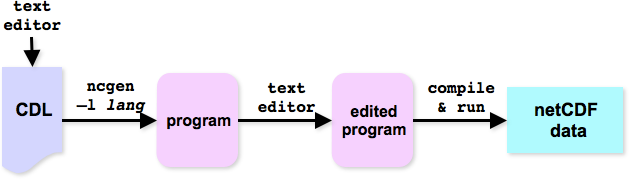
\includegraphics[scale=0.5]{fig/nc-creat}
\end{center}

    \begin{itemize}
    \setlength\itemsep{0.1cm}
      \item Use a text editor to write a CDL file with lots of metadata but little or no data.
      \item Use \texttt{ncgen} to generate corresponding C or Fortran program for writing netCDF.
      \item Insert appropriate netCDF \textbf{var\_put} calls for writing data.
      \item Compile and run program to create netCDF file.
      \item Use \texttt{ncdump} to verify result.
    \end{itemize}

\end{itemize}

\end{frame}

\begin{frame}[fragile]{Using \texttt{ncdump}}

\begin{itemize}

  \item Inspect the file \verb|simple_xy.nc| using \verb|ncdump|\\[0.4cm]

  \begin{itemize}
  \setlength\itemsep{0.5cm}

    \item \verb|ncdump simple_xy.nc|

    \item \lr{Only works like that in my laptop:}

    \item \verb|/home/lucy/netcdf/netcdf-c-4.7.4/ncdump/ncdump simple_xy.nc|

    \item \lr{It should be just ncdump file, but esdm is on my way and I don’t know how to make another link.}

  \end{itemize}

\end{itemize}

\end{frame}

\begin{frame}[fragile]{NetCDF CDL Format}

{\footnotesize

\begin{verbatim}

netcdf simple_xy {
dimensions:
	x = 6 ;
	y = 12 ;
variables:
	int data(x, y) ;
data:

 data =
  0, 1, 2, 3, 4, 5, 6, 7, 8, 9, 10, 11,
  12, 13, 14, 15, 16, 17, 18, 19, 20, 21, 22, 23,
  24, 25, 26, 27, 28, 29, 30, 31, 32, 33, 34, 35,
  36, 37, 38, 39, 40, 41, 42, 43, 44, 45, 46, 47,
  48, 49, 50, 51, 52, 53, 54, 55, 56, 57, 58, 59,
  60, 61, 62, 63, 64, 65, 66, 67, 68, 69, 70, 71 ;
}

\end{verbatim}

}

\end{frame}

\begin{frame}[fragile]{Using \texttt{ncgen}}

\begin{itemize}

  \item Create a NetCDF file using \verb|ncgen| and the CDL output\\[0.4cm]

    \begin{itemize}
    \setlength\itemsep{0.5cm}

      \item \verb|/home/lucy/netcdf/netcdf-c-4.7.4/ncdump/ncdump simple_xy.nc > simple_xy_test.cdl|
      \item \verb|more simple_xy_test.cdl|
      \item \verb|/home/lucy/netcdf/netcdf-c-4.7.4/ncgen/ncgen -b simple_xy_test.cdl|
      \item \verb|cmp simple_xy_test.nc simple_xy.nc|
      \item \lr{Fix ncdump!}

    \end{itemize}

\end{itemize}

\end{frame}

\begin{frame}[fragile]{Creating the C File}

\begin{itemize}
\setlength\itemsep{0.4cm}

  \item Create a C file using \texttt{ncgen} and the CDL output\\[0.4cm]

  \begin{itemize}
  \setlength\itemsep{0.5cm}

    \item \verb|/home/lucy/netcdf/netcdf-c-4.7.4/ncgen/ncgen -lc simple_xy_test.cdl > simple_xy_test.c|
    \item \verb|more simple_xy_test.c|
    \item What is the difference between the files \verb|simple_xy_test.c| and \verb|simple_xy_wr.c|?
    \item \lr{Fix ncgen!}

    \begin{itemize}
      \item \verb|cmp simple_xy_test.c simple_xy_wr.c|
      \item \verb|meld simple_xy_test.c simple_xy_wr.c|
    \end{itemize}

  \end{itemize}

\end{itemize}

\end{frame}

\begin{frame}[fragile]{Starting all over again!}

\begin{itemize}
  \setlength\itemsep{0.5cm}

  \item \verb|gcc -I/home/username/local/include simple_xy_test.c|\\
  \verb|-o simple_xy_test -L/home/username/local/lib -lnetcdf|
  \item \verb|mv simple_xy_test.nc simple_xy_test2.nc|
  \item \verb|./simple_xy_test|
  \item \verb|cmp simple_xy_test.nc simple_xy_test2.nc|

\end{itemize}

\end{frame}

\begin{frame}[fragile]{ncview}

\begin{itemize}

  \item \lr{Installation is fine.}
  \item \lr{What does it do?}

  \begin{center}
  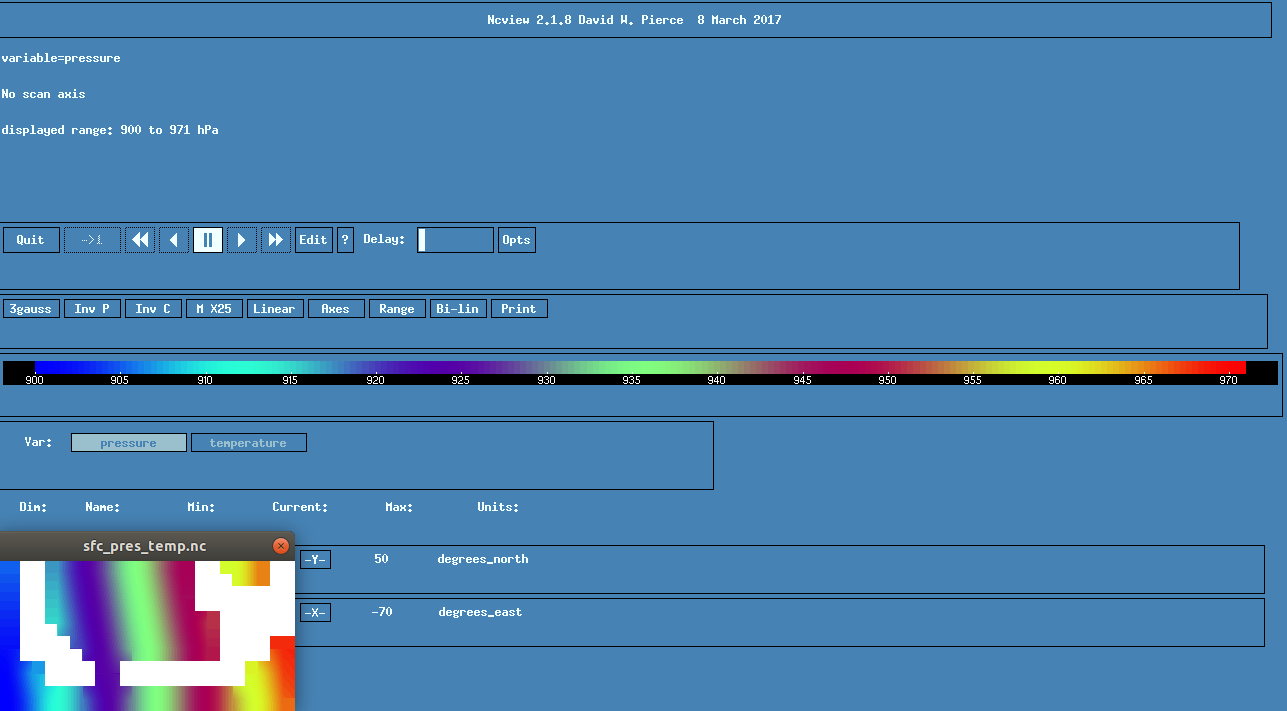
\includegraphics[scale=0.3]{fig/ncview}
  \end{center}

\end{itemize}

\end{frame}

\section{NetCDF Operators}

\begin{frame}[fragile]{NetCDF Operators (NCO)\lr{Is there time to explore?}}

\begin{itemize}

  \item NCO is a package of command line operators that manipulates generic netCDF data and supports some CF conventions. The NCO utilities are:

{ \footnotesize

\begin{table}
\begin{center}
\begin{tabular}{cc}

\begin{tabular}{|l|l|}
\hline
ncap2 & arithmetic processor \\ \hline
ncatted & attribute editor \\ \hline
ncbo & binary operator \\ \hline
ncdiff & differencer \\ \hline
ncea & ensemble averager \\ \hline
ncecat & ensemble concatenator \\ \hline
ncflint & file interpolator \\ \hline
\end{tabular}

&

\begin{tabular}{|l|l|}
\hline
ncks & kitchen sink \\
& (extract, cut, paste, print data) \\ \hline
ncpdq & permute dimensions quickly \\ \hline
ncra & running averager \\ \hline
ncrcat & record concatenator \\ \hline
ncrename & renamer \\ \hline
ncwa & weighted averager \\ \hline
\end{tabular}

\end{tabular}
\end{center}
\end{table}

}

\item NCO utilities have as a goal being as generic as possible, imposing no limitations on data dimensionality, size, or type. All established national and international climate modelling centers now install and maintain NCO for their users for data post-processing, hyper-slabbing, and serving.

\end{itemize}

\end{frame}

\section{Parallel I/O}

\begin{frame}[fragile]{Parallel I/O}

Implement an application that utilises parallel I/O to store and analyse data

\end{frame}

\section{Practising}

\begin{frame}[fragile]{Files for Practising}

\begin{itemize}
%\setlength\itemsep{0.2cm}

  \item {\scriptsize File \verb|simple_xy_nc4|}
    \begin{itemize}
      \item {\scriptsize Write/Read the \verb|simple_xy| file with some of the features of netCDF-4.}
      \item {\tiny \url{https://www.unidata.ucar.edu/software/netcdf/docs/simple__xy__nc4__wr_8c.html}}
      \item {\tiny \url{https://www.unidata.ucar.edu/software/netcdf/docs/simple__xy__nc4__rd_8c.html}}
    \end{itemize}

  \item {\scriptsize File \verb|simple_nc4|}
    \begin{itemize}
      \item {\scriptsize Write/Read a file demonstrating some of the features of netCDF-4.}
      \item {\tiny \url{https://www.unidata.ucar.edu/software/netcdf/docs/simple__nc4__wr_8c.html}}
      \item {\tiny \url{https://www.unidata.ucar.edu/software/netcdf/docs/simple__nc4__rd_8c.html}}
    \end{itemize}

  \item {\scriptsize File \verb|sfc_pres_temp_wr|}
    \begin{itemize}
      \item {\scriptsize This is an example program which writes/reads surface pressure and temperatures.}
      \item {\tiny \url{https://www.unidata.ucar.edu/software/netcdf/docs/sfc__pres__temp__wr_8c.html}}
      \item {\tiny \url{https://www.unidata.ucar.edu/software/netcdf/docs/sfc__pres__temp__rd_8c.html}}
    \end{itemize}

  \item {\scriptsize File \verb|pres_temp_4D_wr|}
    \begin{itemize}
      \item {\scriptsize This is an example program which writes/reads 4D pressure and temperatures.}
      \item {\tiny \url{https://www.unidata.ucar.edu/software/netcdf/docs/pres__temp__4D__wr_8c.html}}
      \item {\tiny \url{https://www.unidata.ucar.edu/software/netcdf/docs/pres__temp__4D__rd_8c.html}}
    \end{itemize}

\end{itemize}

\end{frame}

\begin{frame}[fragile]{Summary of Actions}

\begin{itemize}
\setlength\itemsep{0.3cm}

  \item Inspect the read and write files in C code.
  \item Compile and run the write/read C files.
  \item Inspect the output NetCDF file (.nc) using \texttt{ncdump}.
  \item Create a CDL file for the NetCDF file.
  \item Recreate the NetCDF file using \texttt{ncgen} and the CDL file.
  \item Recreate the C file using \texttt{ncgen} and the CDL file.
  \item Visualize the data in the NetCDF file with \texttt{ncview}.

\end{itemize}

\end{frame}

\section{Starting with NetCDF}
\label{netcdf}

\subsection{Building NetCDF}

\begin{frame}[fragile]{Building NetCDF from Scratch}

\begin{itemize}
\setlength\itemsep{0.8cm}

  \item The usual way of building netCDF requires the HDF5, zlib, and curl libraries.

  \item Files for the libraries can be found in:

\end{itemize}

\begin{center}
\url{ftp://ftp.unidata.ucar.edu/pub/netcdf/netcdf-4}
\end{center}

\end{frame}

\subsection{Installing curl}

\begin{frame}[fragile]{Installing curl}

\begin{itemize}

  \item apt-get install libcurl4-openssl-dev

\end{itemize}

\end{frame}

\subsection{Installing zlib}

\begin{frame}[fragile]{Installing zlib}

\begin{itemize}
\setlength\itemsep{0.3cm}

  \item wget \url{ftp://ftp.unidata.ucar.edu/pub/netcdf/netcdf-4/zlib-1.2.8.tar.gz}
  \begin{itemize}
    \item Newest version to later use ncview
    \item wget \url{https://sourceforge.net/projects/libpng/files/zlib/1.2.9/zlib-1.2.9.tar.gz}
  \end{itemize}
  \item tar -xvzf zlib-1.2.8.tar.gz
  \item cd zlib-1.2.8
  \item mkdir /home/username/local/
  \item ./configure --prefix=/home/username/local/
  \item make check install

\end{itemize}

\end{frame}

\subsection{Installing HDF5}

\begin{frame}[fragile]{Installing HDF5}

\begin{itemize}
\setlength\itemsep{0.3cm}

  \item wget \url{ftp://ftp.unidata.ucar.edu/pub/netcdf/netcdf-4/hdf5-1.8.13.tar.gz}
  \item tar -xvzf hdf5-1.8.13.tar.gz
  \item cd hdf5-1.8.13
  \item ./configure --with-zlib=/home/username/local/ --prefix=/home/username/local/
  \item make
  \item make check
  \item make install
  \begin{itemize}
    \item make check install
    \item If not done separately, it might not work!
  \end{itemize}
\end{itemize}

\end{frame}

\subsection{Installing NetCDF}

\begin{frame}[fragile]{Installing NetCDF}

\begin{itemize}
\setlength\itemsep{0.3cm}

  \item Check the latest version at \url{https://www.unidata.ucar.edu/downloads/netcdf/}
  \item wget \url{ftp://ftp.unidata.ucar.edu/pub/netcdf/netcdf-c-4.7.4.tar.gz}
  \item tar -xvzf netcdf-c-4.7.4.tar.gz
  \item cd netcdf-c-4.7.4
  \item CPPFLAGS=-I/home/username/local/include LDFLAGS=-L/home/username/local/lib ./configure --prefix=/home/username/local
  \item make check install

\end{itemize}

\end{frame}

\begin{frame}[fragile]{Finishing the Set Up}

\begin{itemize}
\setlength\itemsep{0.8cm}
  \item Link the NetCDF library\\
  \begin{itemize}
  \setlength\itemsep{0.2cm}
    \item export \verb|LD_LIBRARY_PATH=/home/username/local/lib/|
    \item \verb|sudo ldconfig|
  \end{itemize}
  \item Create a new directory (for instance, /home/username/example) and create the file from the given source using an editor of your choice.

\end{itemize}

\end{frame}

\subsection{File \texttt{simple\_xy\_wr.c}}

% Inserting [fragile] to be able to work with \verb

\begin{frame}[fragile]{File Reference: \texttt{simple\_xy\_wr.c}}

This is an example program demonstrating a simple 2D write. It is intended to illustrate the use of the netCDF C API.\\[0.3cm]

\begin{itemize}
  \item {\tiny \url{https://www.unidata.ucar.edu/software/netcdf/docs/simple__xy__wr_8c.html}}\\[0.3cm]
  \item {\tiny \url{https://www.unidata.ucar.edu/software/netcdf/docs/simple__xy__wr_8c_source.html}}\\[0.4cm]
\end{itemize}

Dependency graph for \verb|simple_xy_wr|:

\begin{center}
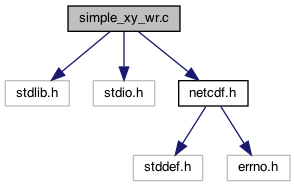
\includegraphics[scale=0.5]{fig/simple__xy__wr_8c__incl}
\end{center}

\end{frame}

\subsection{Working and analysing the NetCDF File}

\begin{frame}[fragile]{Compiling and running the file \texttt{simple\_xy\_wr.c}}

\begin{itemize}
\setlength\itemsep{0.6cm}

  \item Create (copy!) and compile the file \verb|simple_xy_wr.c|.

    \begin{itemize}
      \item {\tiny \verb|gcc -I/home/username/local/include simple_xy_wr.c -o simple_xy_wr -L/home/username/local/lib -lnetcdf|}
    \end{itemize}

  \item Run the file \verb|simple_xy_wr|.

      \begin{itemize}
        \item {\tiny  \verb|./simple_xy_wr|}
        \item {\tiny  \verb|*** SUCCESS writing example file simple_xy.nc!|}\\[0.5cm]
      \end{itemize}

  \item Check that the file \verb|cmp test.nc simple_xy.nc| is in your directory.

\end{itemize}

\end{frame}

\begin{frame}[fragile]{Using \texttt{ncdump}}

Inspect the output file \verb|simple_xy.nc| using \verb|ncdump|

\begin{itemize}

  \item \verb|ncdump simple_xy.nc|

  \item \lr{Only works like that in my laptop:}

  \item \verb|/home/lucy/netcdf/netcdf-c-4.7.4/ncdump/ncdump simple_xy.nc|

  \item \lr{It should be just ncdump file, but esdm is on my way and I don’t know how to make another link}

\end{itemize}

\end{frame}

\begin{frame}[fragile]{NetCDF CDL Format}

{\footnotesize

\begin{verbatim}

netcdf simple_xy {
dimensions:
	x = 6 ;
	y = 12 ;
variables:
	int data(x, y) ;
data:

 data =
  0, 1, 2, 3, 4, 5, 6, 7, 8, 9, 10, 11,
  12, 13, 14, 15, 16, 17, 18, 19, 20, 21, 22, 23,
  24, 25, 26, 27, 28, 29, 30, 31, 32, 33, 34, 35,
  36, 37, 38, 39, 40, 41, 42, 43, 44, 45, 46, 47,
  48, 49, 50, 51, 52, 53, 54, 55, 56, 57, 58, 59,
  60, 61, 62, 63, 64, 65, 66, 67, 68, 69, 70, 71 ;
}

\end{verbatim}

}

\end{frame}

\begin{frame}[fragile]{Using \texttt{ncgen}}

\begin{itemize}

  \item Create a NetCDF file using \verb|ncgen| and the CDL output

    \begin{itemize}

      \item \verb|/home/lucy/netcdf/netcdf-c-4.7.4/ncdump/ncdump simple_xy.nc > test.cdl|
      \item \verb|more test.cdl|
      \item \verb|/home/lucy/netcdf/netcdf-c-4.7.4/ncgen/ncgen -b test.cdl|
      \item \verb|cmp test.nc simple_xy.nc|
      \item \lr{Fix ncdump!}

    \end{itemize}

\end{itemize}

\end{frame}

\begin{frame}[fragile]{Creating the C File}

\begin{itemize}
\setlength\itemsep{0.5cm}

  \item Create a C file using ncgen and the CDL output

    \begin{itemize}

      \item \verb|/home/lucy/netcdf/netcdf-c-4.7.4/ncgen/ncgen -lc simple_xy_test.cdl > simple_xy_test.c|
      \item \verb|more simple_xy_test.c|
      \item \verb|cmp simple_xy_test.c simple_xy_wr.c|
      \item \lr{Fix ncgen!}

    \end{itemize}

\end{itemize}

\end{frame}

\begin{frame}[fragile]{Starting all over again!}

\begin{itemize}

  \item \verb|gcc -I/home/username/local/include simple_xy_test.c -o simple_xy_test -L/home/username/local/lib -lnetcdf|
  \item \verb|mv simple_xy_test.nc simple_xy_test2.nc|
  \item \verb|./simple_xy_test|
  \item \verb|cmp simple_xy_test.nc simple_xy_test2.nc|

\end{itemize}

\end{frame}

\begin{frame}[fragile]{File Reference: \texttt{simple\_xy\_rd.c}}

This is a simple example which reads a small dummy array, which was written by \verb|simple_xy_wr.c|. It is intended to illustrate the use of the netCDF C API.\\[0.3cm]

\begin{itemize}
  \item {\tiny \url{https://www.unidata.ucar.edu/software/netcdf/docs/simple__xy__rd_8c.html}}\\[0.3cm]
  \item {\tiny \url{https://www.unidata.ucar.edu/software/netcdf/docs/simple__xy__rd_8c_source.html}}\\[0.4cm]
\end{itemize}

Dependency graph for \verb|simple_xy_wr|:

\begin{center}
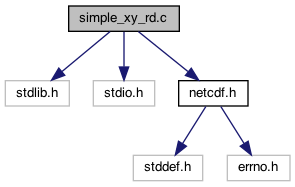
\includegraphics[scale=0.5]{fig/simple__xy__rd_8c__incl}
\end{center}

\end{frame}

\begin{frame}[fragile]{Reading the file \texttt{simple\_xy.nc}}

\begin{itemize}
\setlength\itemsep{0.6cm}

  \item Check that the file \verb|simple_xy.nc| is in your directory.

  \item Create (copy!), compile and run the file \verb|simple_xy_rd.c|\\[0.4cm]

        \begin{itemize}
          \item {\tiny  \verb|gcc -I/home/username/local/include simple_xy_rd.c -o simple_xy_rd -L/home/username/local/lib -lnetcdf| }\\[0.4cm]
        \end{itemize}

  \item Run the file \verb|simple_xy_rd|

        \begin{itemize}

          \item {\tiny  \verb|./simple_xy_rd|}

          \item {\tiny  \verb|*** SUCCESS reading example file simple_xy.nc!|}

        \end{itemize}

\end{itemize}

\end{frame}

\begin{frame}[fragile]{ncview}

\begin{itemize}

  \item Installation is fine.
  \item What does it do?

\end{itemize}

\begin{center}
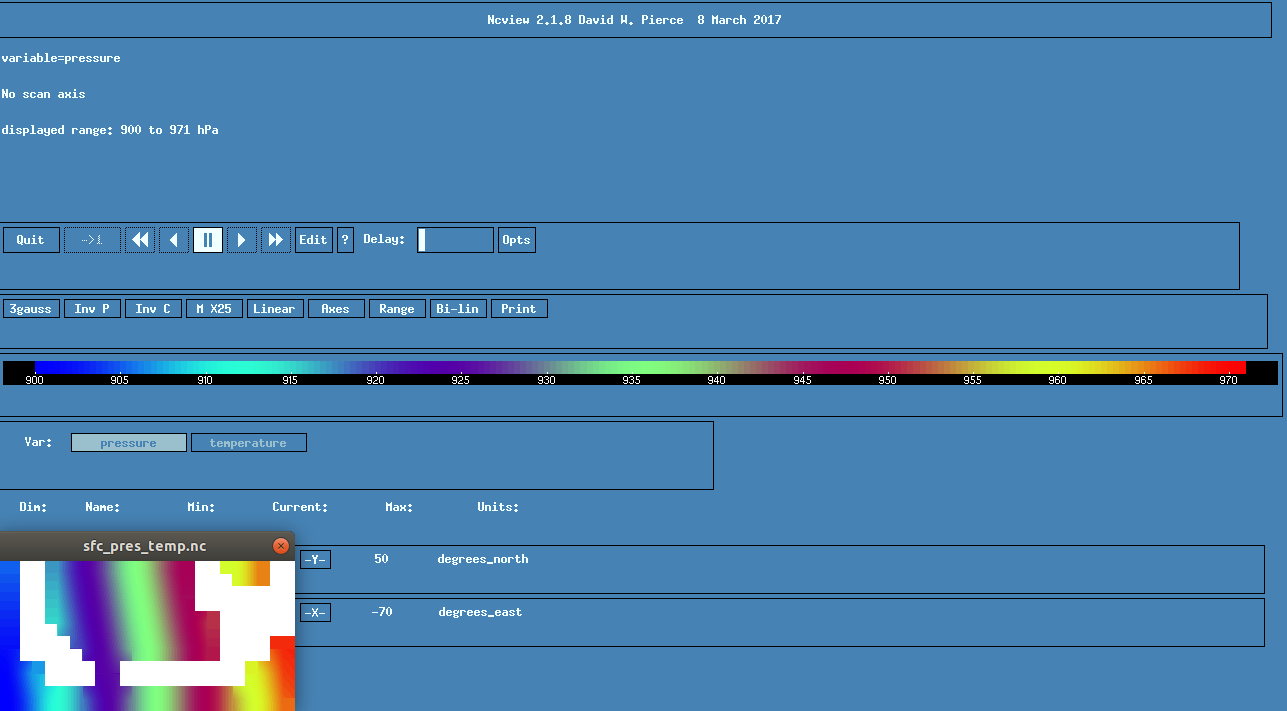
\includegraphics[scale=0.3]{fig/ncview}
\end{center}

\end{frame}

\acknowledgement

\end{document}
